% =====================================================================
%  MEDUSA – Verarbeitungspipeline (einreihig, Labels über den Boxen)
%
%  Benötigte TikZ-Bibliotheken (im Hauptdokument):
%      \usetikzlibrary{arrows.meta, positioning, calc, fit, backgrounds}
% =====================================================================

\providecommand{\stagenum}[1]{{\footnotesize\bfseries\color{blue!55!black}#1}}
\providecommand{\stagettl}[1]{{\scriptsize\bfseries\shortstack[c]{#1}}}

\begin{tikzpicture}[
    >=Latex,
    node distance=0.5cm,
    every node/.style={font=\footnotesize},
    %
    stage/.style={
        rectangle, rounded corners=3pt,
        draw=blue!55!black, thick,
        top color=blue!4, bottom color=blue!14,
        minimum width=2.0cm, minimum height=2.0cm,
        align=center, inner sep=3pt,
    },
    flow/.style={->, line width=0.7pt, draw=blue!55!black},
    flowlabel/.style={
        font=\scriptsize, text=black!75,
        inner xsep=2pt, inner ysep=1pt, align=center,
    },
    iolabel/.style={font=\scriptsize\bfseries, text=black!75, align=center},
    viz/.style={
        rectangle, rounded corners=3pt,
        draw=green!45!black, thick, dashed,
        fill=green!6, inner sep=6pt, align=center,
    },
    vizflow/.style={->, dashed, line width=0.6pt, draw=green!45!black},
]
% --------------------------- Stufen ----------------------------------
\node[stage] (s1) {%
    \stagenum{1}\\[1pt]\stagettl{Schicht-\\positionen}\\[4pt]
    \begin{tikzpicture}[baseline]
        \draw[gray!55] (0,0) rectangle (0.55,0.4);
        \foreach \y in {0.08,0.20,0.32}
            \draw[blue!65!black, thin] (-0.04,\y) -- (0.59,\y);
    \end{tikzpicture}};

\node[stage, right=of s1] (s2) {%
    \stagenum{2}\\[1pt]\stagettl{Schnitt}\\[4pt]
    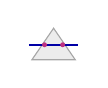
\begin{tikzpicture}[baseline]
        \fill[gray!15] (0,0)--(0.55,0)--(0.275,0.4)--cycle;
        \draw[gray!70] (0,0)--(0.55,0)--(0.275,0.4)--cycle;
        \draw[blue!65!black, thick] (-0.04,0.19)--(0.59,0.19);
        \fill[magenta!75!black] (0.16,0.19) circle (0.9pt);
        \fill[magenta!75!black] (0.39,0.19) circle (0.9pt);
    \end{tikzpicture}};

\node[stage, right=of s2] (s3) {%
    \stagenum{3}\\[1pt]\stagettl{Verkettung}\\[4pt]
    
\begin{tikzpicture}[baseline]
        \draw[magenta!75!black, very thick, rounded corners=1pt]
            (0.07,0.10)--(0.20,0.05)--(0.38,0.05)--
            (0.50,0.15)--(0.50,0.28)--(0.38,0.37)--
            (0.20,0.37)--(0.07,0.28)--cycle;
    \end{tikzpicture}};

\node[stage, right=of s3] (s4) {%
    \stagenum{4}\\[1pt]\stagettl{Reihenfolge}\\[4pt]
    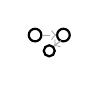
\begin{tikzpicture}[baseline]
        \draw[thick] (0.10,0.30) circle (0.08);
        \draw[thick] (0.46,0.30) circle (0.08);
        \draw[thick] (0.28,0.10) circle (0.07);
        \draw[->, thin, gray!70, dashed] (0.19,0.30)--(0.37,0.30);
        \draw[->, thin, gray!70, dashed] (0.43,0.23)--(0.34,0.16);
    \end{tikzpicture}};

\node[stage, right=of s4] (s5) {%
    \stagenum{5}\\[1pt]\stagettl{Emission}\\[4pt]
    
\begin{tikzpicture}[baseline]
        \draw[gray!70] (0.05,0) rectangle (0.52,0.4);
        \foreach \y in {0.08,0.16,0.24,0.32}
            \draw[gray!55, thin] (0.10,\y)--(0.47,\y);
    \end{tikzpicture}};

% --------------------------- Datenfluss-Pfeile -----------------------
\draw[flow] (s1.east) -- (s2.west);
\draw[flow] (s2.east) -- (s3.west);
\draw[flow] (s3.east) -- (s4.west);
\draw[flow] (s4.east) -- (s5.west);

% --------------------------- Labels ÜBER den Boxen -------------------
\node[flowlabel, above=2pt]
    at ($(s1.north east)!0.5!(s2.north west)$) {Höhen $a_i$};
\node[flowlabel, above=2pt]
    at ($(s2.north east)!0.5!(s3.north west)$) {Segmente};
\node[flowlabel, above=2pt]
    at ($(s3.north east)!0.5!(s4.north west)$) {Konturringe};
\node[flowlabel, above=2pt]
    at ($(s4.north east)!0.5!(s5.north west)$) {geordnete Ringe};

% --------------------------- I/O -------------------------------------
\draw[flow] ([xshift=-0.8cm]s1.west) -- (s1.west);
\node[iolabel, anchor=east] at ([xshift=-0.85cm]s1.west) {\gls{mesh}};

\draw[flow] (s5.east) -- ([xshift=0.8cm]s5.east);
\node[iolabel, anchor=west] at ([xshift=0.85cm]s5.east)
    {Schicht-\\datensatz};

% --------------------------- Viz-Box ---------------------------------
\node[viz,
      fit={(s1.south west) (s5.south east)},
      inner xsep=6pt, inner ysep=10pt,
      minimum height=1.1cm,
      yshift=-1.3cm] (vizfit)
    {\textbf{\footnotesize Visualisierung}~\scriptsize(3D-Viewer, OpenGL)\\[3pt]%
     \scriptsize\itshape read-only Zugriff auf jede Pipeline-Stufe};

\foreach \s in {s1,s2,s3,s4,s5}
    \draw[vizflow] (\s.south) -- (\s.south |- vizfit.north);

\end{tikzpicture}